\documentclass[tikz]{standalone}
\usepackage{tikz}
\usepackage{mathpazo}
\usetikzlibrary{positioning,calc}
%\usetikzlibrary{matrix}

\definecolor{nodecolor}{HTML}{9999AA}

\tikzset{basic/.style={draw,fill=nodecolor!20,text width=1em,text badly centered}}
\tikzset{input/.style={basic,circle,node distance=3em}}
\tikzset{weights/.style={basic,rectangle}}
\tikzset{functions/.style={basic,circle,fill=nodecolor!10}}
\tikzset{every left delimiter/.style={xshift=0.7em,font=\scriptsize}}

\begin{document}
    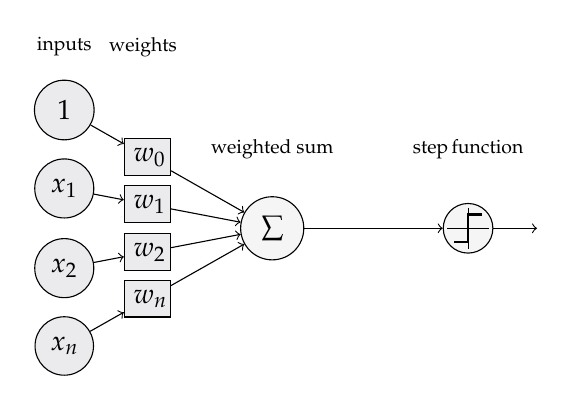
\begin{tikzpicture}

        % Activation function
        \node[functions] (step) {};
        \draw[thick] (0.5em,0.5em) -- (0,0.5em) -- (0,-0.5em) -- (-0.5em,-0.5em);
        \draw (0em,0.75em) -- (0em,-0.75em);
        \draw (0.75em,0em) -- (-0.75em,0em);

        % Arrow pointing to the right
        \node[right of=step] (right) {};
        \path[draw,->] (step) -- (right);

        % Sum function
        \node[functions,left=5em of step] (sum) {$\sum$};
        \path[draw,->] (sum) -- (step);

        % Inputs
        \node[left=6em of sum,text width=0em] (imid) {};
        \node[input,below=0em of imid] (i2) {$x_2$};
        \node[input,above=0em of imid] (i1) {$x_1$};
        \node[input,above=0.65em of i1] (i0) {$1$};
        \node[input,below=0.65em of i2] (in) {$x_n$};

        % Weights
        \node[weights] at ($(i0)!0.4!(sum)$) (w0) {$w_0$} -- (i0);
        \node[weights] at ($(i1)!0.4!(sum)$) (w1) {$w_1$} -- (i1);
        \node[weights] at ($(i2)!0.4!(sum)$) (w2) {$w_2$} -- (i2);
        \node[weights] at ($(in)!0.4!(sum)$) (wn) {$w_n$} -- (in);

        % Remaining arrows
        \draw[->] (i0) -- (w0);
            \path[draw,->] (w0) -- (sum);
        \path[draw,->] (i1) -- (w1);
            \path[draw,->] (w1) -- (sum);
        \path[draw,->] (i2) -- (w2);
            \path[draw,->] (w2) -- (sum);
        \path[draw,->] (in) -- (wn);
            \path[draw,->] (wn) -- (sum);

                % Labels
        \node[above=0.5em of i0,font=\scriptsize] (li) {inputs};
        \node[right of=li,font=\scriptsize] (lw) {weights};
        \node[above of=sum,font=\scriptsize] {weighted sum};
        \node[above of=step,font=\scriptsize] {step\,function};

        % Formulas
        %\node[below=2em of sum,font=\scriptsize] (fsum) {$\sum\limits_{i=0}^n w_i \cdot x_i$};
        %\matrix[matrix of math nodes,below=2em of
        %    step,xshift=0.7em,font=\scriptsize,left delimiter=\lbrace,text width=4em] (fstep) {
        %    & 1 \textrm{~~~if } s \ge 0 \\
        %    & 0 \textrm{~~~otherwise} \\
        %};

    \end{tikzpicture}
\end{document}
